% Chapter Template

\chapter{Related Work} % Main chapter title

\label{Chapter2} % Change X to a consecutive number; for referencing this chapter elsewhere, use \ref{ChapterX}

\lhead{Chapter 2. \emph{Related Work}} % Change X to a consecutive number; this is for the header on each page - perhaps a shortened title

%----------------------------------------------------------------------------------------

% Several attempts have been made in the past to measure the internet traffic.

In this section, we'll review the work done on internet measurement. It has been further subdivided into two sections. The first section talks about the measurements done using P4 programmable switches by the P4Campus group at Princeton. The second section talks about other internet measurements done to better our understanding of transport protocols.

\section{P4Campus at Princeton}

\begin{figure}[t]
    \centering
        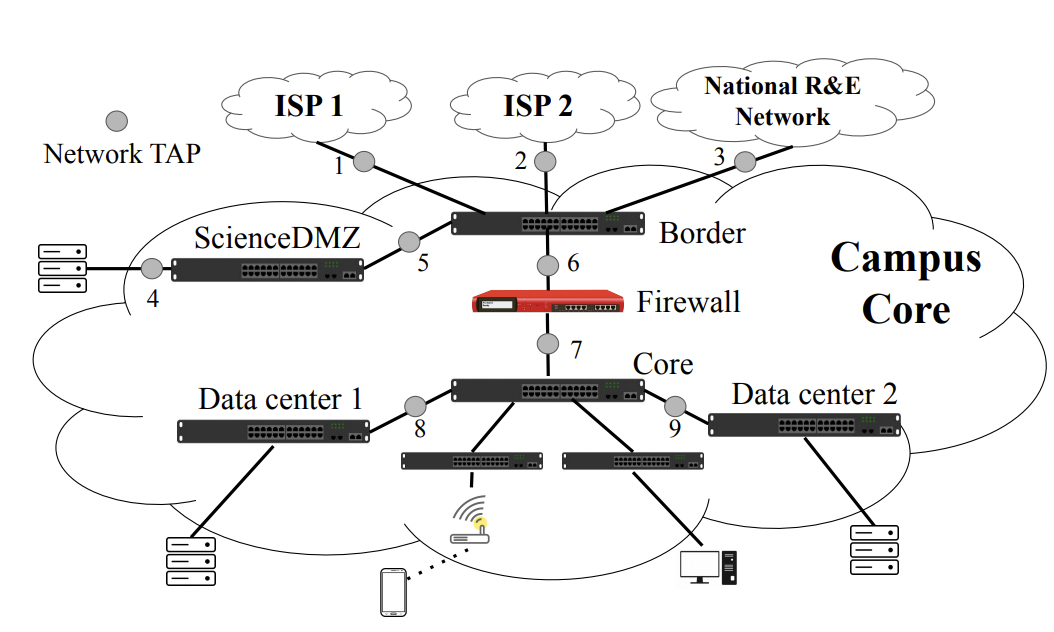
\includegraphics[width=\textwidth]{Figures/image.png}
    \caption[P4Campus]{P4Campus ~\cite{p4campusprinceton}}
    \label{fig:p4camp}
    \bigskip
\end{figure}

The P4Campus project~\cite{p4campusprinceton} at Princeton University is very similar to our CampusMeasure project in terms of the setup used. The backbone of their setup is the same as ours. Figure \ref{fig:p4camp} shows the key differences between the two setups. They have tapped the links at multiple points, whereas we tap the links at only one point(at the gateway router). They use a custom anonymization policy ONTAS~\cite{ontas-netai19} which performs line rate anonymization of traffic, with the option of encrypting ethernet and IP headers on programmable switches using P4. They also don't perform payload truncation contrary to our policy.

Their group has made several measurements over the years with the help of their setup in their campus network. The group focuses on implementing systems in the data plane using the P4~\cite{p4lang} language to make measurements. Dart~\cite{dart-sigcomm22} is a system that performs continuous in-network RTT estimation in the data plane by passively measuring internet traffic. The system maintains a packet-tracker table, by creating an entry in a hash table using the four-tuple of the flow and the expected ACK number as the key, and the timestamp as the value. It then matches the corresponding ACK packet and measures the RTT by calculating the difference in the two timestamps. The system also avoids ambiguous RTT measurements caused due to packet losses and re-ordering, by maintaining a range tracker table for each flow. The range tracker maintains a valid range of sequence numbers for a flow and collapses the range in case of a packet loss or re-transmission event. Oliver et al.~\cite{zoom-imc22} perform passive measurements on Zoom's custom RTP header to measure fine-grained metrics like media-bit rates, delay-frame rates, frame-level jitter, and retransmission. They perform an entropy-based packet header analysis for an RTP packet by plotting the header values on a graph for different packets, in order to decipher different fields of the unknown packet. Sherry et al.~\cite{osfingerprint-netsoft22} performed experiments to fingerprint operating systems on commodity switches passively to detect OS-specific vulnerabilities and administer OS-related security policies that block, rate-limit, or redirect traffic. They determine OS-specific fingerprints based on the TCP and IP header values of a packet. Upon encountering a packet, they match the TCP and IP header values with the existing signatures to determine the OS. The TCP options are used for more specific fingerprinting. Jason et al.~\cite{domainnameanalysis-sosr21} characterize traffic using high-level indicators like domain name instead of IP address in the data plane. They extract the domain names queried by clients by tracking the DNS response packets along with the client and server IP addresses and store them in a hash table. They then keep track of the count of the data packets from the server to the client to measure the traffic volume per flow. Chen et al.~\cite{conquest-conext19} perform fine-grained queue measurement to identify flows contributing to queue(FIFO) buildup and latency. The routers are tapped on both ends to determine the arrival and departure times of the packets. They measure the queuing delay for a packet by capturing the arrival and departure times, and if the delay is greater than a certain threshold, they check for flows contributing to the queue buildup. The percentage of packets of each flow in the queue is calculated and flows contributing to queue buildup are reported. Ben-Basat et al.~\cite{probabilisticrecirculation-icnp2018} find heavy hitter flows in the queues by using counter-based algorithms. They maintain a hash table to count the number of packets per flow and increment the counter each time a packet of the flow arrives. If the flow is not already present in the hash table, they probabilistically re-circulate the packet to avoid processing delay each time, per the high switch speed. If in case the table is full, the flow with the minimum count is evicted.

\section{Other Internet measurement techniques}

RTT measurements on the internet traffic have been made since a long time. Some of the most fundamental tools like ping~\cite{iputils} and traceroute~\cite{inetutils} use active measurement techniques to measure RTT for a flow. Active measurement techniques may not always produce accurate results as they might increase congestion in an already congested network. Studies have shown that the RTT measurements made by ping are not very accurate because of flow-level load balancing done by network routers, resulting in different traffic routes for ICMP ping packets ~\cite{paris2tokyoping-imc13}. Passive measurement of RTT done by analysing the TCP handshake might not be enough as shown by Jay et al.~\cite{tcprtt-imc03}. They recorded one of the first RTT measurements passively between endpoints at a large university campus.Their studies showed that the RTT values vary widely over a time for a long flow. Shakkottai et al. ~\cite{2004-shakkottai-t20} measured the RTT distribution of TCP flows using different methods and its impact on TCP-based flow control.

Feng et al. ~\cite{tcprevisited-imc09} determine the initial congestion window size, irregular retransmission events and TCP flow clocking by analyzing uni-directional TCP flows. They calculate the ICW size using an algorithm that identifies the first large gap between the sending of two packets by the server. They also detect irregular retransmissions by the sender. by statistically checking if there is a negative correlation between the retransmission rate and the sending rate. They extract the TCP flow clock from the uni-directional trace using Fourier transforms.  Raman et al.~\cite{tampering-sigcomm23} detect connection tampering done by middleboxes by passively comparing TCP flows with certain tampering signatures. The tampering signatures are a comprehensive list of sequences of TCP header packets that are indicative of a tampering event. Some of the frequent signatures observed by them were tampering mid-TCP handshake and immediately after the TCP handshake. Debopam et al.~\cite{latency-imc20} reconstructed licensed financial trading networks to examine their latency, wireless link lengths, path redundancy, and other features. Benko et al.~\cite{1189102} calculate packet losses passively by using the TCP sequence numbers and noticing the retransmissions and re-ordering events. They refine their measurements by calculating loss rates only for significant packets and ignoring the packets for which the loss is too uncertain like the first and last data segments of a flow and re-transmitted packets. Joel et al.~\cite{10.1145/1090191.1080111}
tried improving the accuracy in end-to-end packet loss measurement using active probes by Zing~\cite{707817}, a tool that sends UDP packets at Poisson-modulated intervals with a fixed mean rate.
%----------------------------------------------------------------------------------------